\section{Silicon --- valence and low lying conduction states}
\label{sec11:silicon}

\begin{figure}[h!]
\centering
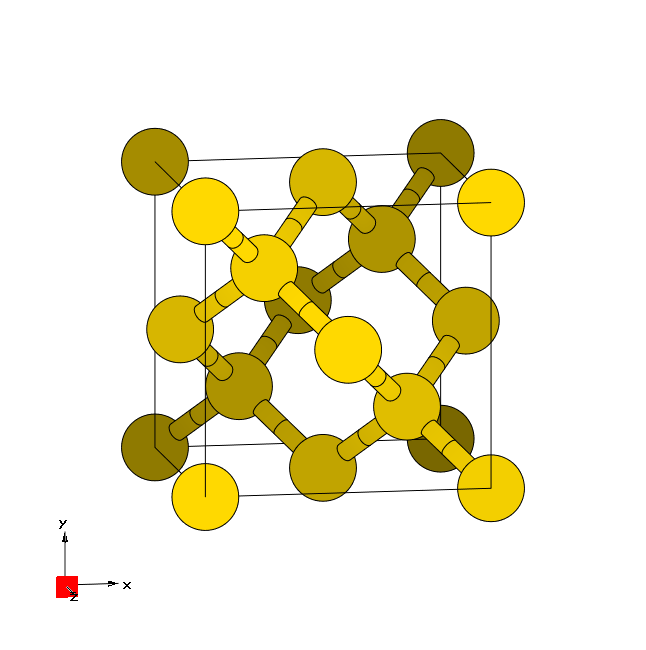
\includegraphics[width=0.25\columnwidth,trim={45pt 45pt 55pt 55pt},clip]{figure/example11/silicon.png}
\caption{Unit cell of Silicon crystal plotted with the \xcrysden{} program.}
\label{fig11.0}
\end{figure}

\subsection*{Valence States}
\begin{itemize}
\item Outline: {\it Obtain MLWFs for the valence bands of silicon.}
\end{itemize}


\begin{itemize}
	\item[1-5] {\it Inspect the output file {\tt silicon.wout}. The total spread converges to its minimum value after just a
few iterations. Note that the geometric centre of each MLWF lies at the centre of the Si--Si bond. Note
also that the memory requirement for the minimisation of the spread is very low as the MLWFs are
defined by just the $4\times4$ unitary matrices $U(\mathbf{k})$.}

Below a snippet from the {\tt silicon.wout} output file
  \begin{tcolorbox}[sharp corners,boxrule=0.5pt]
  {\small
\begin{verbatim}
 Final State
  WF centre and spread    1  ( -0.674701,  0.674701, -0.674701 )     1.59185520
  WF centre and spread    2  ( -0.674701, -0.674701,  0.674701 )     1.59185520
  WF centre and spread    3  (  0.674701,  0.674701,  0.674701 )     1.59185520
  WF centre and spread    4  (  0.674701, -0.674701, -0.674701 )     1.59185520
  Sum of centres and spreads ( -0.000000,  0.000000,  0.000000 )     6.36742081

         Spreads (Ang^2)       Omega I      =     5.801375426
        ================       Omega D      =     0.000000000
                               Omega OD     =     0.566045385
    Final Spread (Ang^2)       Omega Total  =     6.367420811
 ------------------------------------------------------------------------------
\end{verbatim}
}
\end{tcolorbox}
Memory estimates may be found in the {\tt MEMORY ESTIMATE} section of the {\tt silicon.wout} file.
  \begin{tcolorbox}[sharp corners,boxrule=0.5pt]
  {\small
\begin{verbatim}
 *============================================================================*
 |                              MEMORY ESTIMATE                               |
 |         Maximum RAM allocated during each phase of the calculation         |
 *============================================================================*
 |                        Disentanglement            1.57 Mb                  |
 |                            Wannierise:            0.47 Mb                  |

\end{verbatim}
}
\end{tcolorbox}
Converged values for the total spread functional and its components are shown in Tab.~\ref{tab11.1}.

\begin{table}[t!]
\centering
\caption{Converged values of the components of spread functional and their sum, given in \angsqd{}.}
\begin{tabular}{@{} lllll @{}}\toprule[1.5pt]
MP mesh & $\Omega$ & $\Omega\tinysub{I}$ & $\Omega\tinysub{OD}$ & $\Omega\tinysub{D}$ \\\midrule
$4\times4\times4$ & 6.3674  &  5.8014 & 0.5660 & 0.0000 \\\bottomrule
\end{tabular}\label{tab11.1}
\end{table}

\item {\it Plot the MLWFs}
The four MLWFs with $\sigma$ character describing the valence manifold of Si are shown in \Fig{fig11.1}(a),(b) and (c) respectively.
	\begin{figure}[h!]
	\centering
	\subfloat[1]{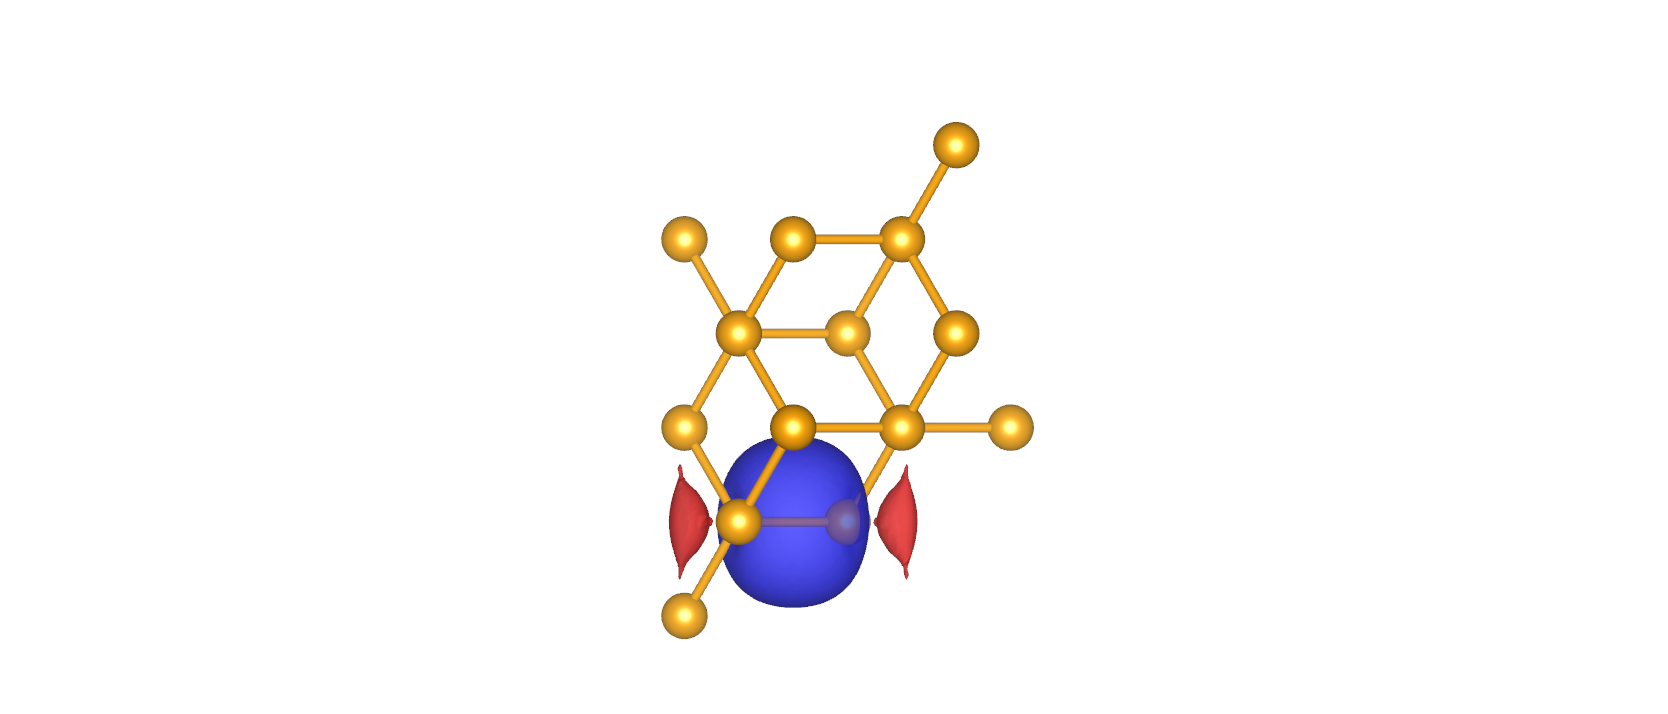
\includegraphics[width=0.25\columnwidth,trim={500pt 0pt 500pt 0pt},clip]{figure/example11/silicon_valence_1.png}}
	\centering
	\subfloat[2]{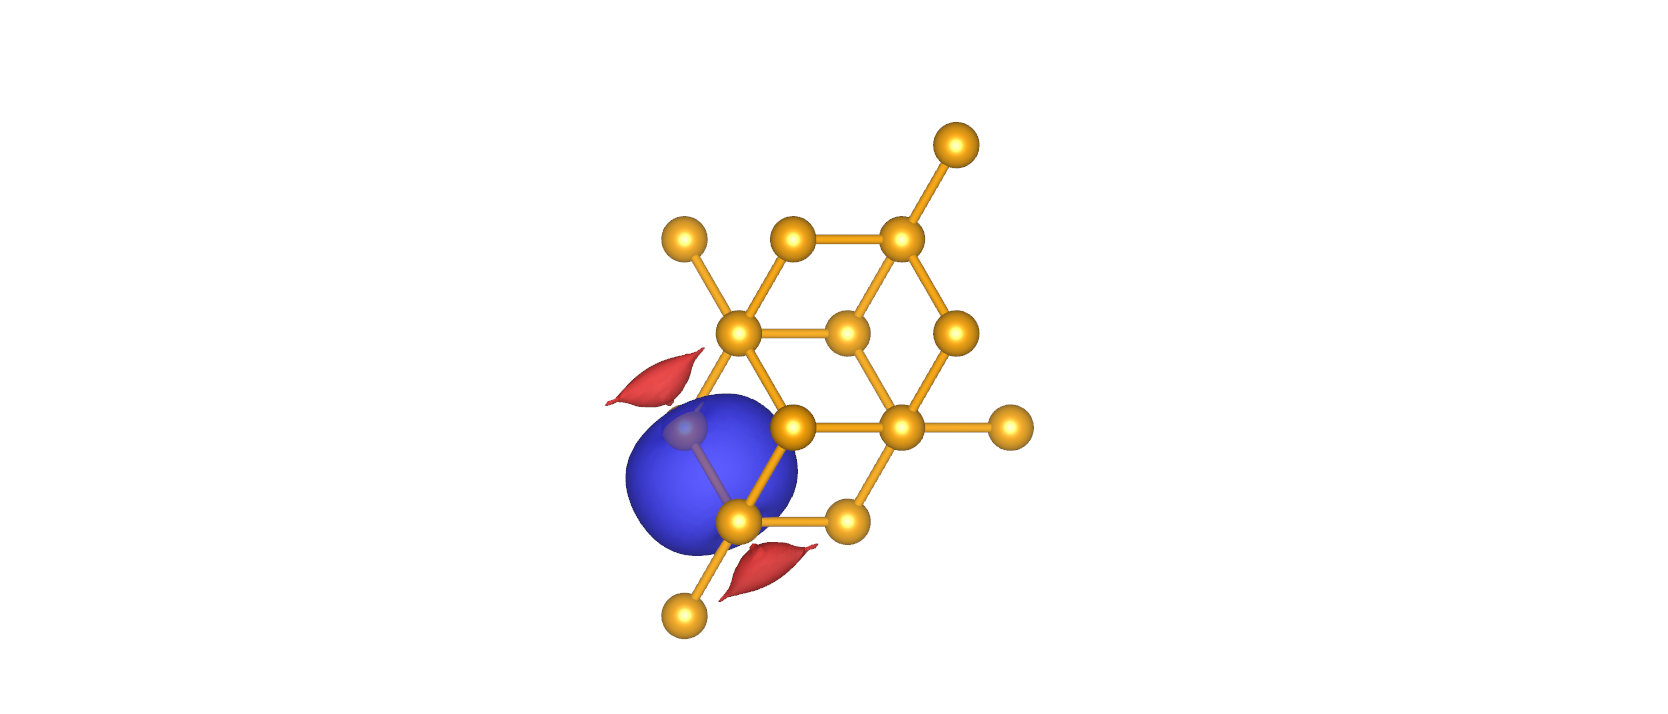
\includegraphics[width=0.25\columnwidth,trim={500pt 0pt 500pt 0pt},clip]{figure/example11/silicon_valence_2.png}}
	\centering
	\subfloat[3]{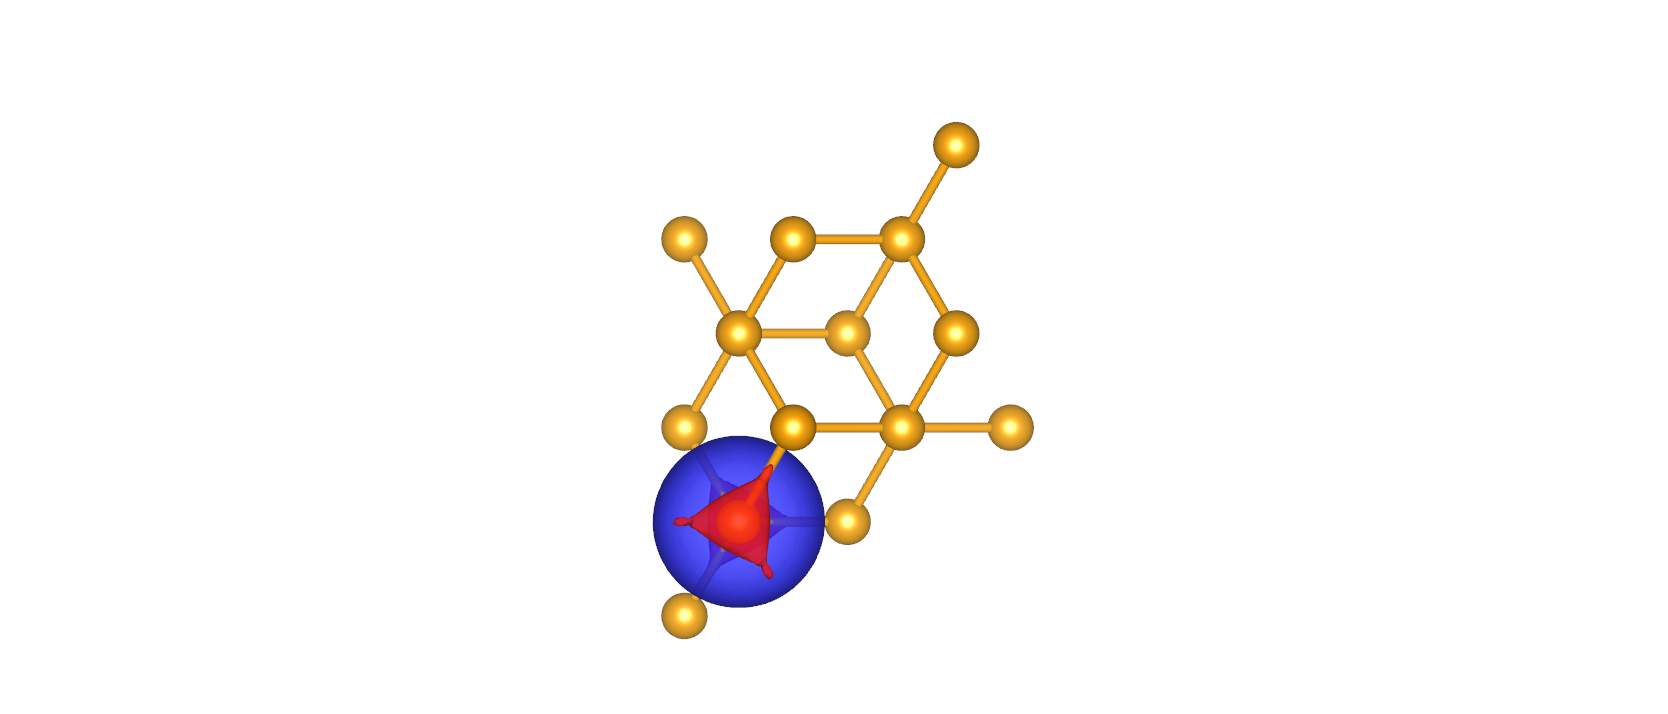
\includegraphics[width=0.25\columnwidth,trim={500pt 0pt 500pt 0pt},clip]{figure/example11/silicon_valence_3.png}}
	\centering
	\subfloat[4]{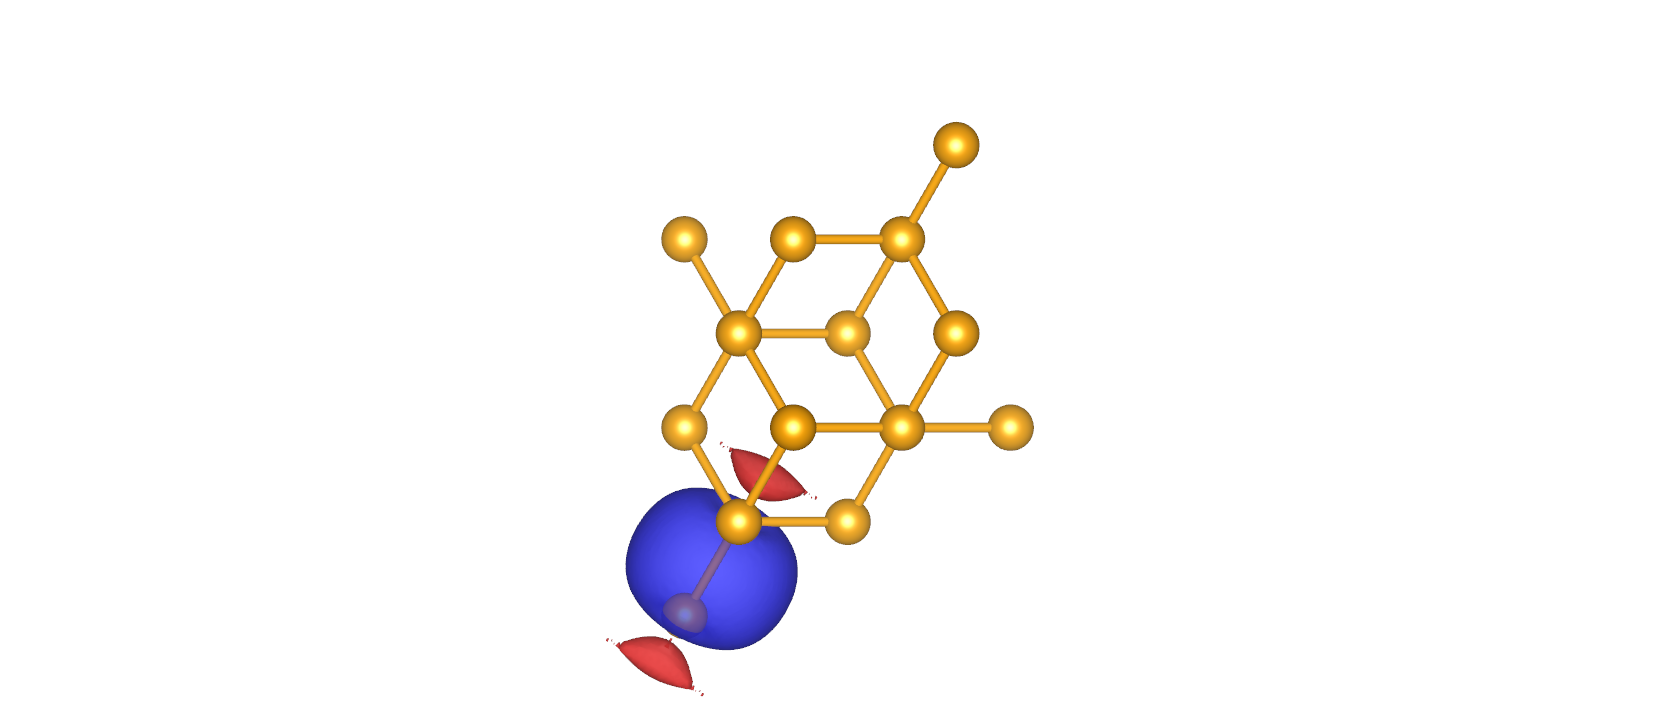
\includegraphics[width=0.25\columnwidth,trim={500pt 0pt 500pt 0pt},clip]{figure/example11/silicon_valence_4.png}}
	\caption{Four MLWFs for the valence manifold of Si.}\label{fig11.1}
	\end{figure}

\end{itemize}
\newpage
\subsection*{Valence + Conduction States}
\begin{itemize}
\item Outline: {\it Obtain MLWFs for the valence and low--lying conduction-band states of Si. Plot the
interpolated bandstructure. Apply a scissors correction to the conduction bands.}
\end{itemize}

\begin{itemize}
	\item {\it Inspect the output file {\tt silicon.wout}. The minimisation of the spread occurs in a two-step procedure. First, we minimise $\Omega\tinysub{I}$ -- this is the extraction of the optimal subspace in the disentanglement procedure. Then, we minimise $\Omega\tinysub{D} + \Omega\tinysub{OD}$.}

	Converged values for the total spread functional and its components are shown in Tab.~\ref{tab11.2}.
	The two groups of four MLWFs with $sp3$ character are shown in \Fig{fig11.2}

	\begin{tcolorbox}[sharp corners,boxrule=0.5pt]
	{\small
	\begin{verbatim}
                   Extraction of optimally-connected subspace
                   ------------------------------------------
 +---------------------------------------------------------------------+<-- DIS
 |  Iter     Omega_I(i-1)      Omega_I(i)      Delta (frac.)    Time   |<-- DIS
 +---------------------------------------------------------------------+<-- DIS
       1      12.97640155      12.44630235       4.259E-02      0.00    <-- DIS
       .		.					.				.			 .

      79      12.33580893      12.33580893      -6.531E-11      0.23    <-- DIS
      80      12.33580893      12.33580893      -5.241E-11      0.23    <-- DIS

             <<<      Delta < 1.000E-10  over  3 iterations     >>>
             <<< Disentanglement convergence criteria satisfied >>>

        Final Omega_I    12.33580893 (Ang^2)

 +----------------------------------------------------------------------------+
	\end{verbatim}
	}
	\end{tcolorbox}

	\begin{tcolorbox}[sharp corners,boxrule=0.5pt]
	{\small
	\begin{verbatim}
	 Final State
  WF centre and spread    1  (  1.807167,  1.807167,  1.807167 )     2.01695824
  WF centre and spread    2  (  1.807167,  0.891636,  0.891636 )     2.01695823
  WF centre and spread    3  (  0.891636,  1.807167,  0.891636 )     2.01695823
  WF centre and spread    4  (  0.891636,  0.891636,  1.807167 )     2.01695824
  WF centre and spread    5  (  0.226733,  0.226733,  0.226733 )     2.37014516
  WF centre and spread    6  (  0.226733, -0.226733, -0.226733 )     2.37014508
  WF centre and spread    7  ( -0.226733,  0.226733, -0.226733 )     2.37014515
  WF centre and spread    8  ( -0.226733, -0.226733,  0.226733 )     2.37014514
  Sum of centres and spreads (  5.397608,  5.397608,  5.397608 )    17.54841346

         Spreads (Ang^2)       Omega I      =    12.335808933
        ================       Omega D      =     0.177593840
                               Omega OD     =     5.035010692
    Final Spread (Ang^2)       Omega Total  =    17.548413465
 ------------------------------------------------------------------------------
 	\end{verbatim}
 	}

	\end{tcolorbox}


	\begin{table}[t!]
	\centering
	\caption{Converged values of the components of spread functional and their sum, given in \angsqd{}.}
	\begin{tabular}{@{} lllll @{}}\toprule[1.5pt]
	MP mesh & $\Omega$ & $\Omega\tinysub{I}$ & $\Omega\tinysub{OD}$ & $\Omega\tinysub{D}$ \\\midrule
	$4\times4\times4$ & 17.54841 &  12.3358 & 5.03501 & 0.17759 \\\bottomrule
	\end{tabular}\label{tab11.2}
	\end{table}

	\begin{figure}[h!]
	\centering
	\subfloat[1]{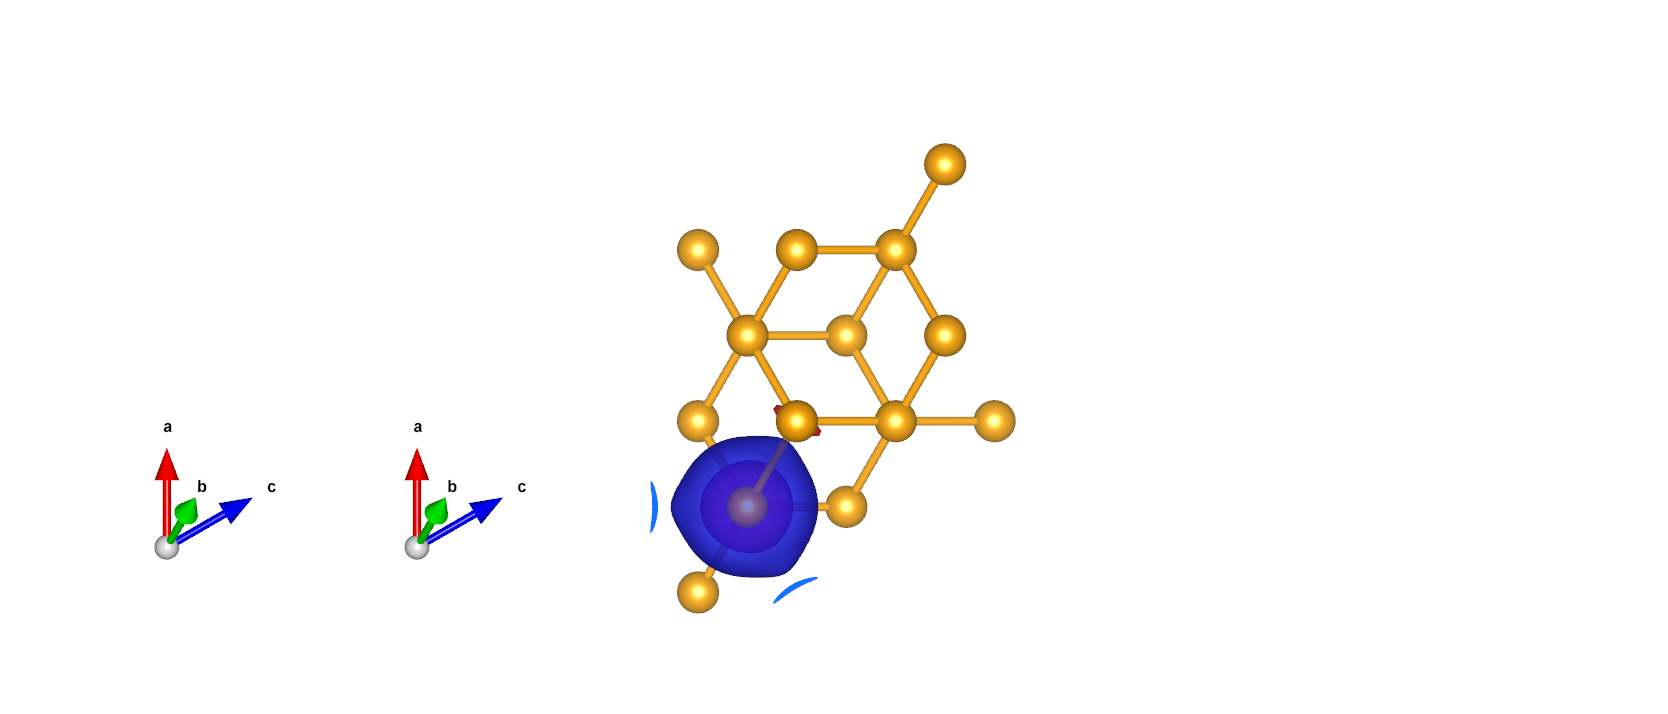
\includegraphics[width=0.25\columnwidth,trim={300pt 0pt 500pt 0pt},clip]{figure/example11/silicon_v+c_1.png}}
	\centering
	\subfloat[2]{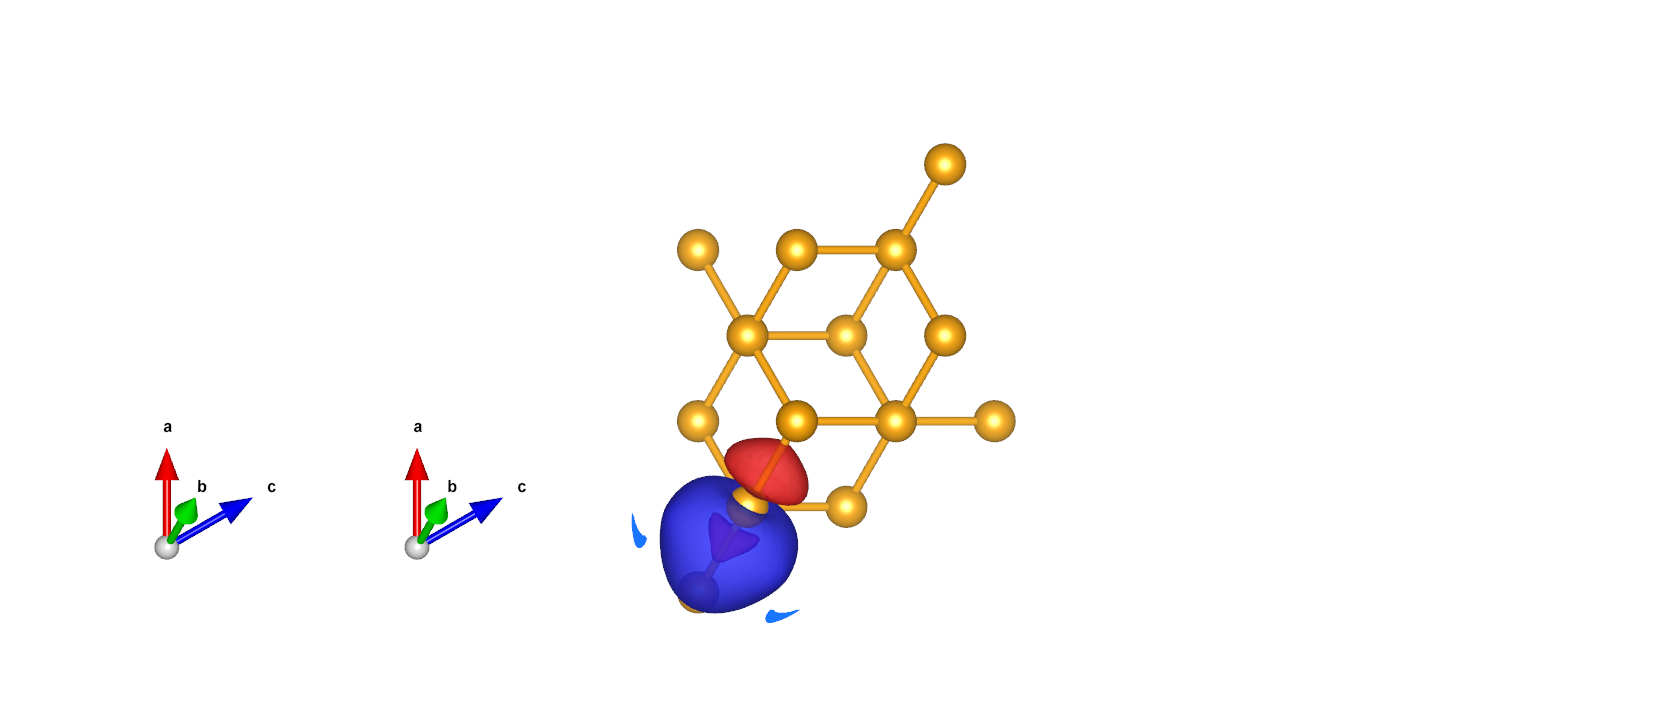
\includegraphics[width=0.25\columnwidth,trim={300pt 0pt 500pt 0pt},clip]{figure/example11/silicon_v+c_2.png}}
	\centering
	\subfloat[3]{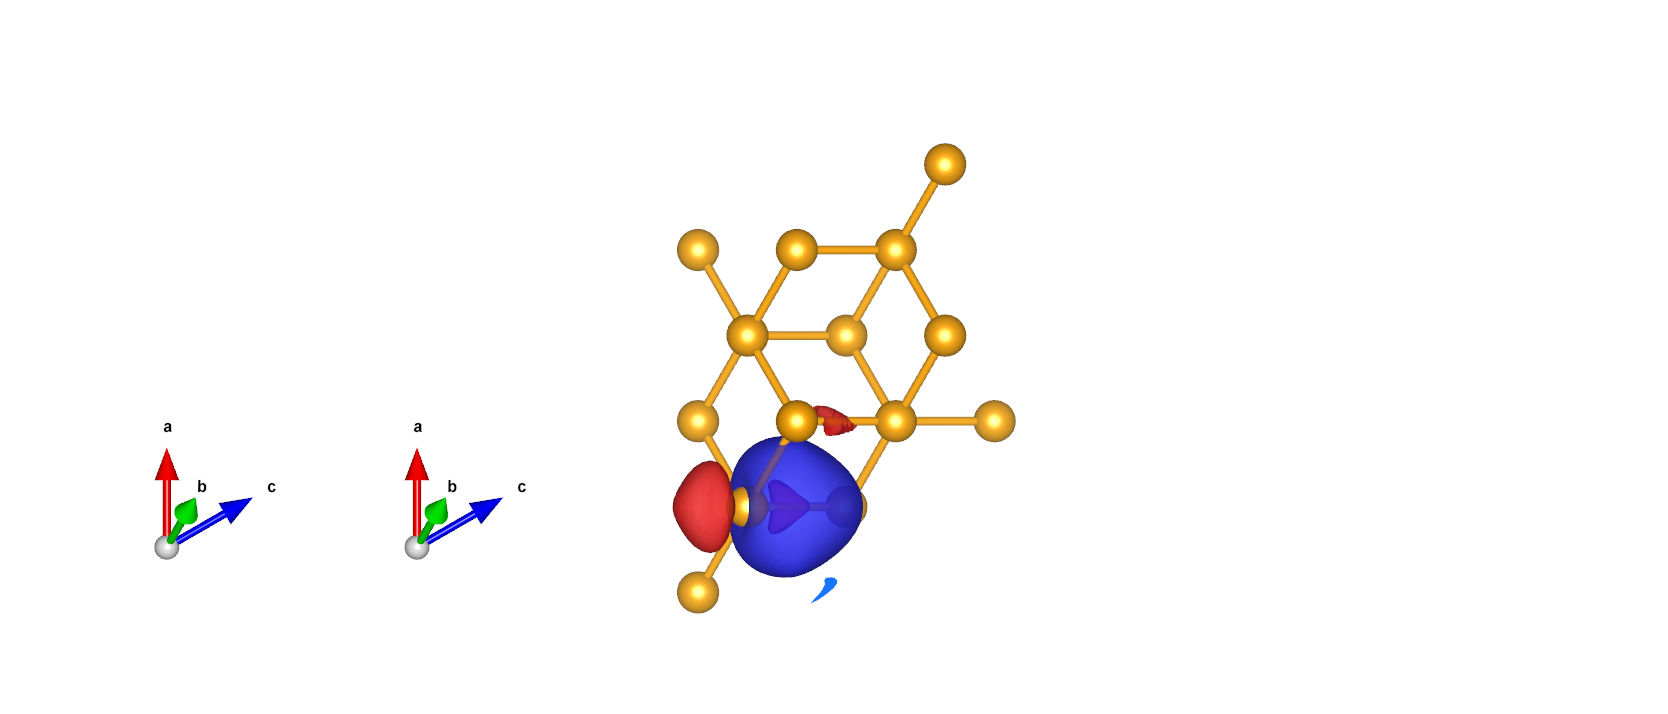
\includegraphics[width=0.25\columnwidth,trim={300pt 0pt 500pt 0pt},clip]{figure/example11/silicon_v+c_3.png}}
	\centering
	\subfloat[4]{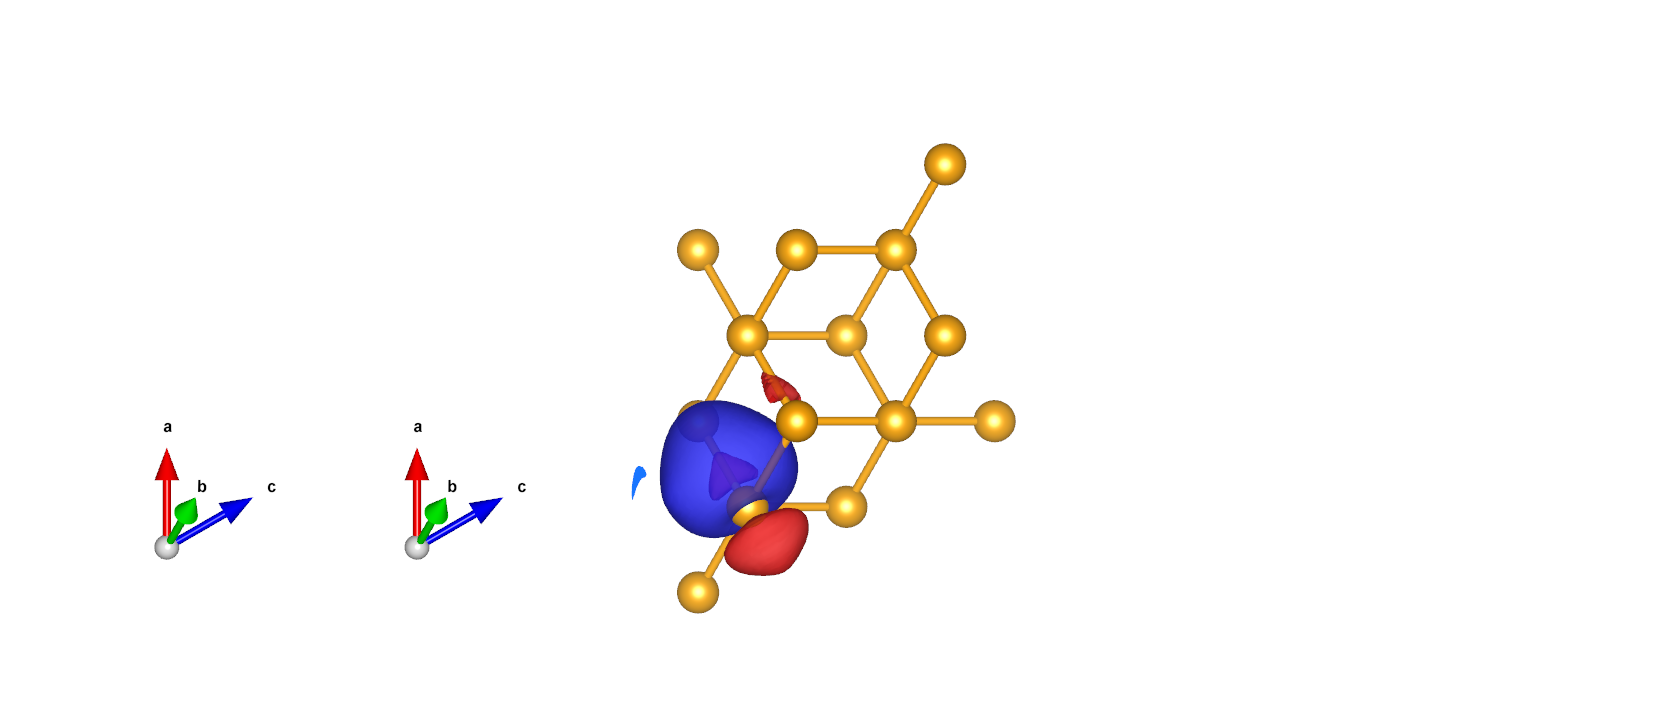
\includegraphics[width=0.25\columnwidth,trim={300pt 0pt 500pt 0pt},clip]{figure/example11/silicon_v+c_4.png}}\\
	\centering
	\subfloat[5]{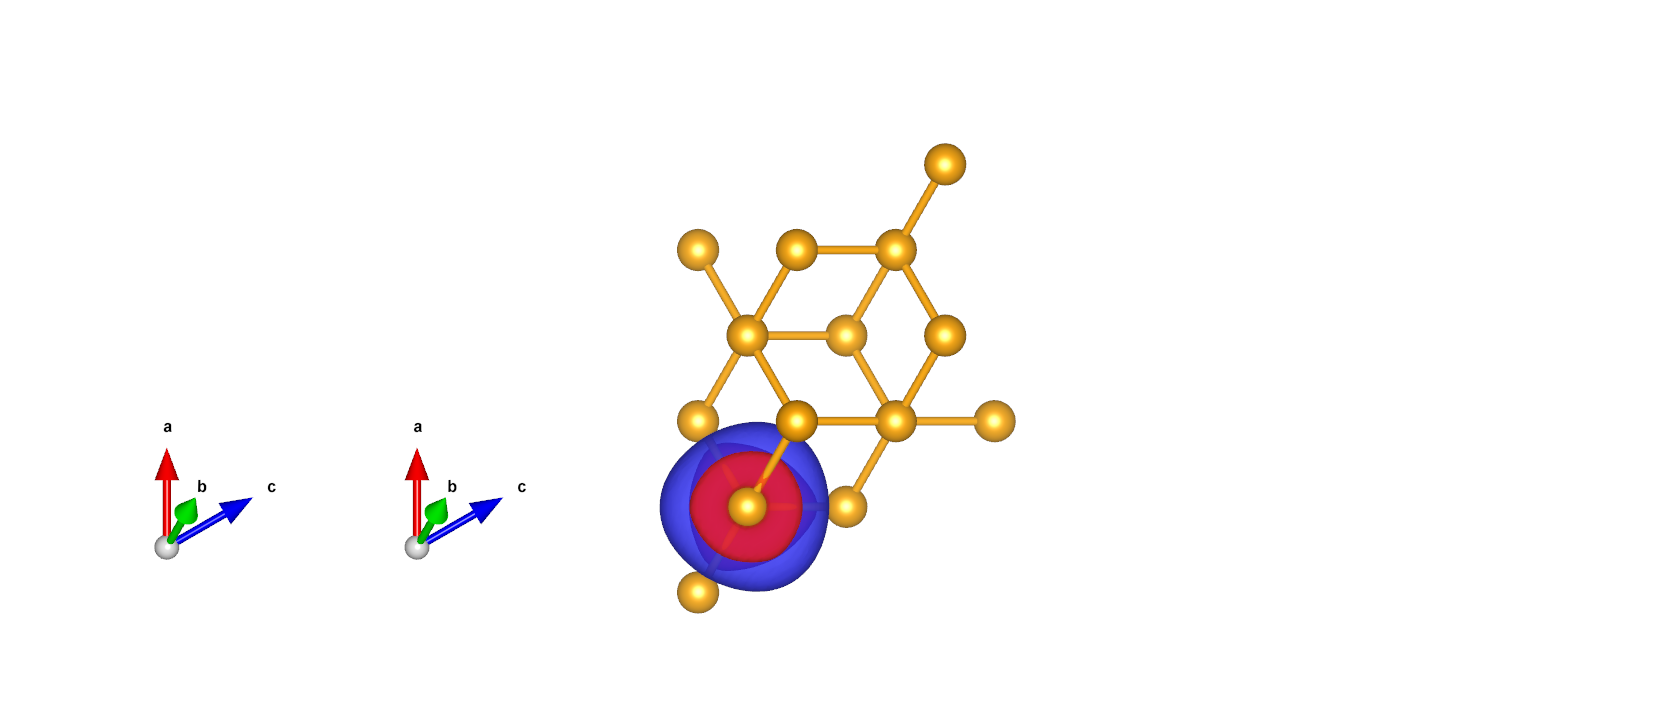
\includegraphics[width=0.25\columnwidth,trim={300pt 0pt 500pt 0pt},clip]{figure/example11/silicon_v+c_5.png}}
	\centering
	\subfloat[6]{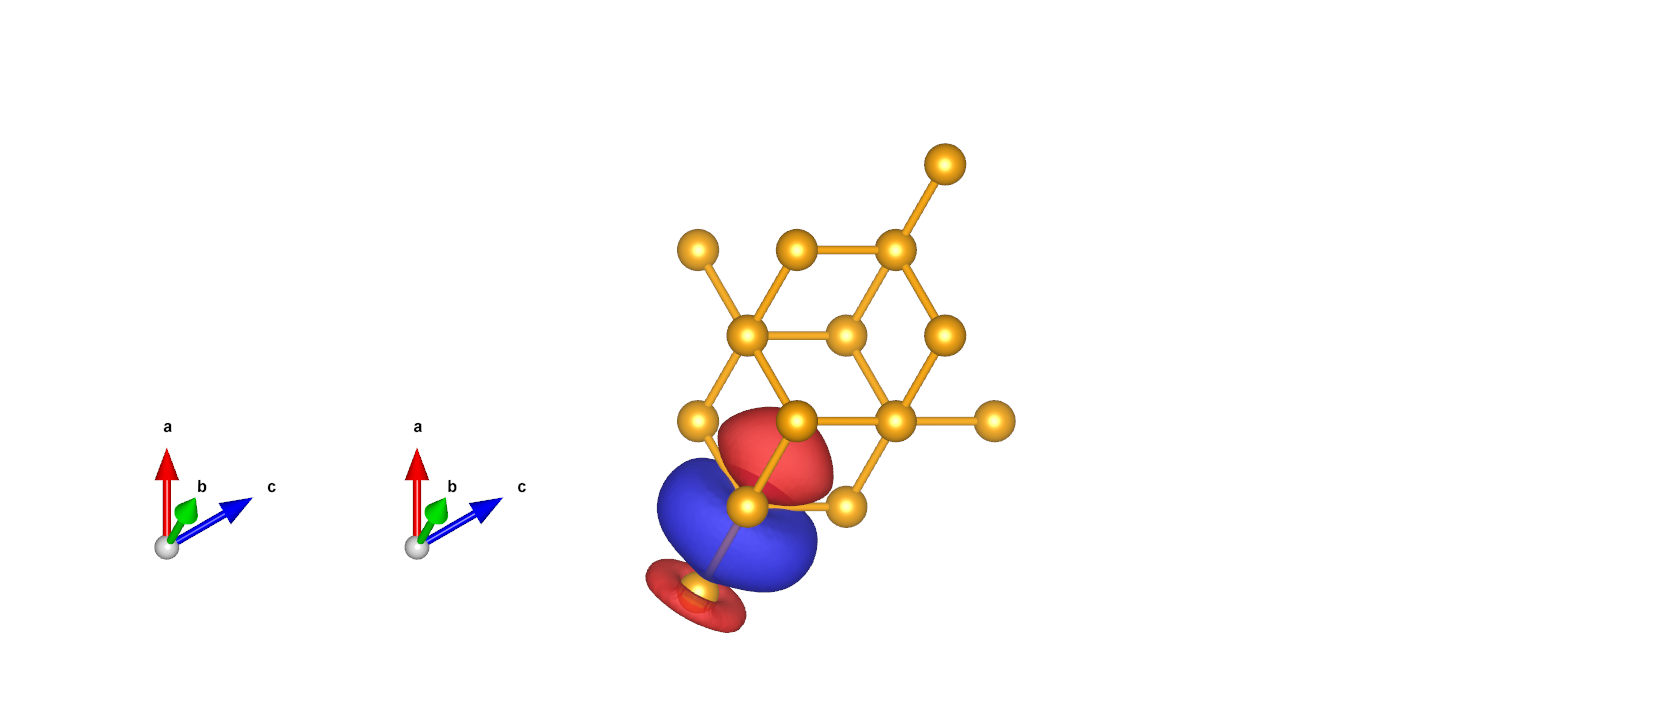
\includegraphics[width=0.25\columnwidth,trim={300pt 0pt 500pt 0pt},clip]{figure/example11/silicon_v+c_6.png}}
	\centering
	\subfloat[7]{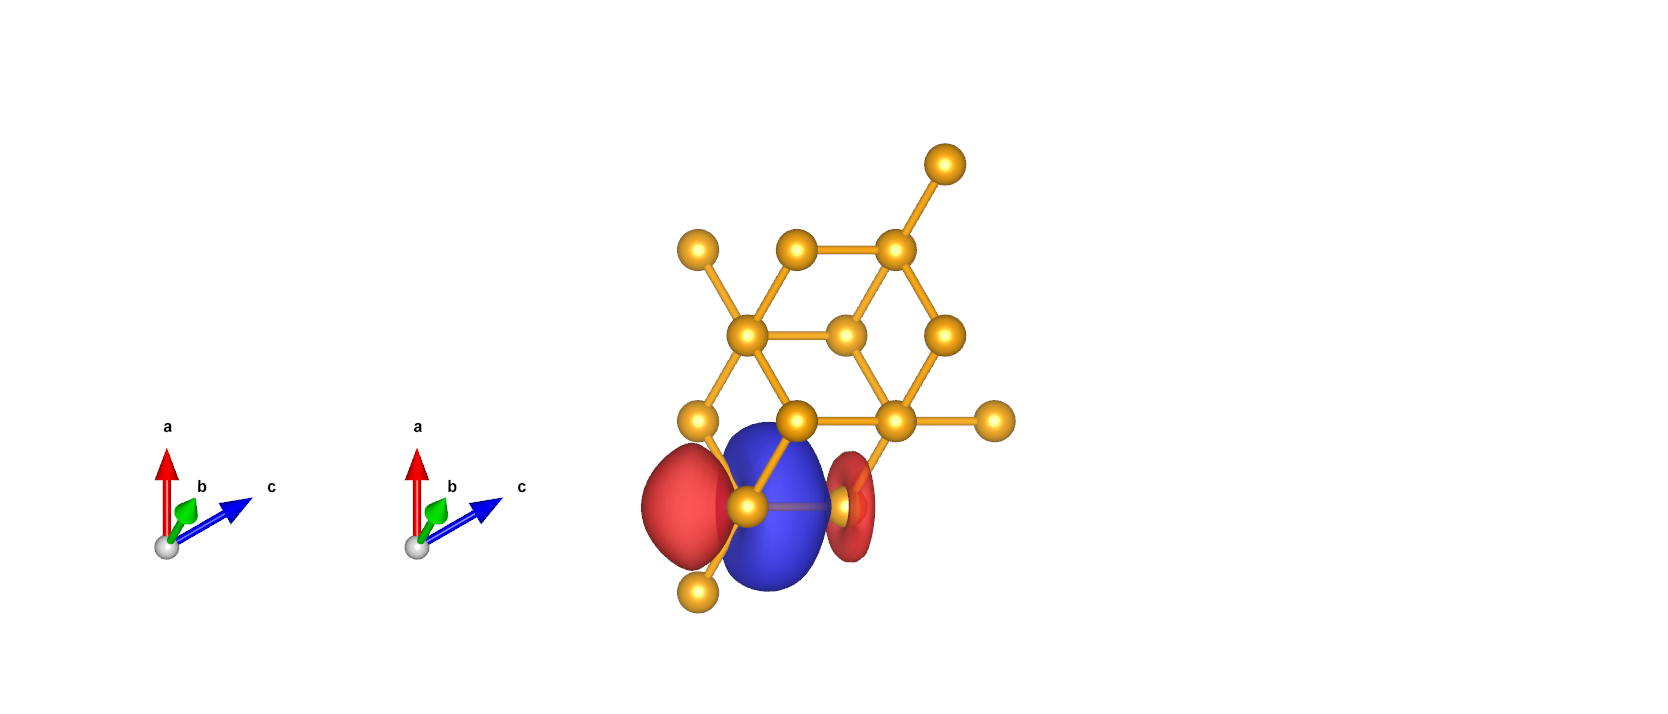
\includegraphics[width=0.25\columnwidth,trim={300pt 0pt 500pt 0pt},clip]{figure/example11/silicon_v+c_7.png}}
	\centering
	\subfloat[8]{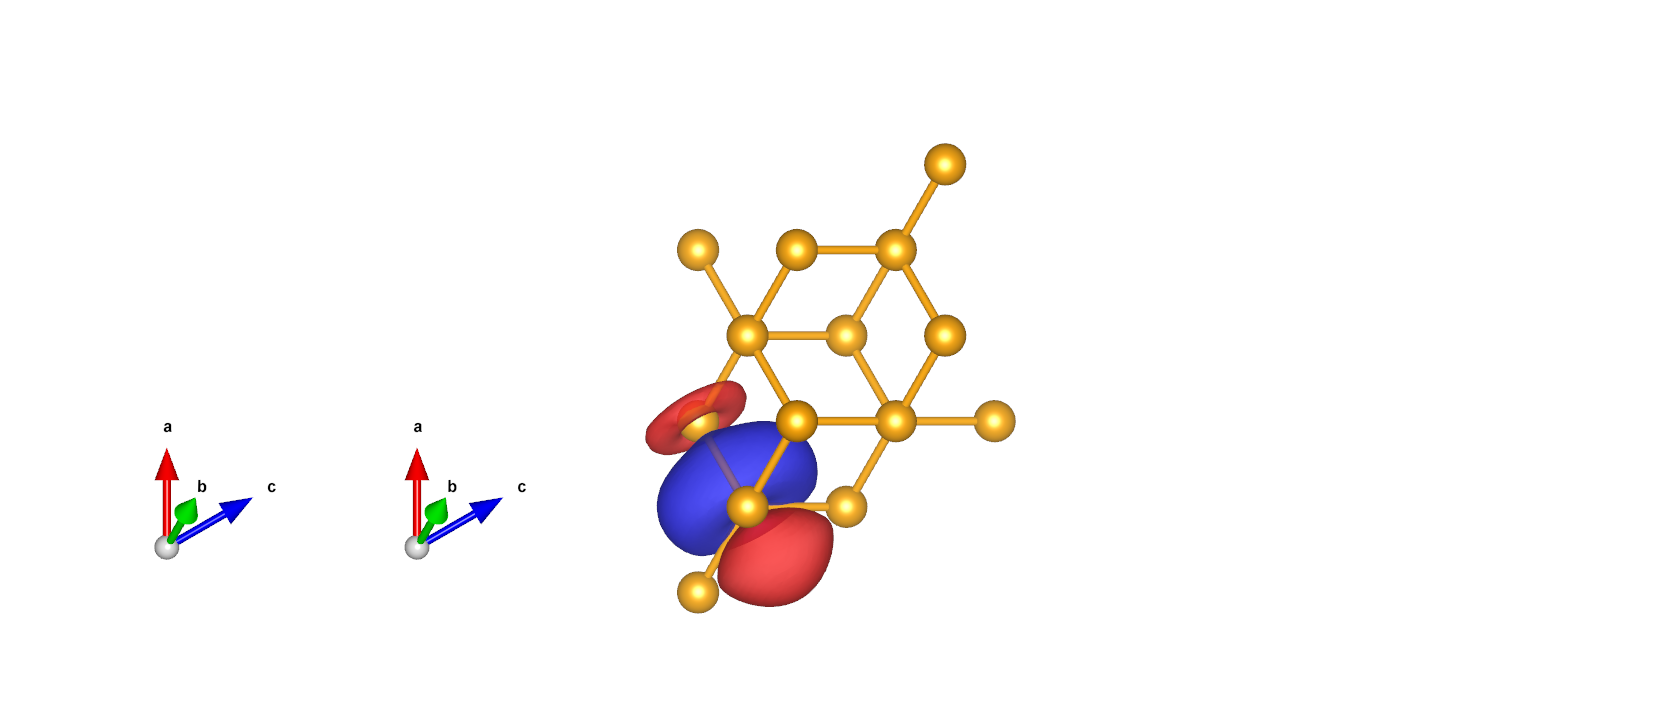
\includegraphics[width=0.25\columnwidth,trim={300pt 0pt 500pt 0pt},clip]{figure/example11/silicon_v+c_8.png}}
	\caption{Eight MLWFs with $sp3$ character, four on each Si atom in the unit cell.}\label{fig11.2}
	\end{figure}
\item {\it Plot the bandstructure.} 

The interpolated bandstructure is given in \Fig{fig11.3}.
\begin{figure}[h!]
\centering
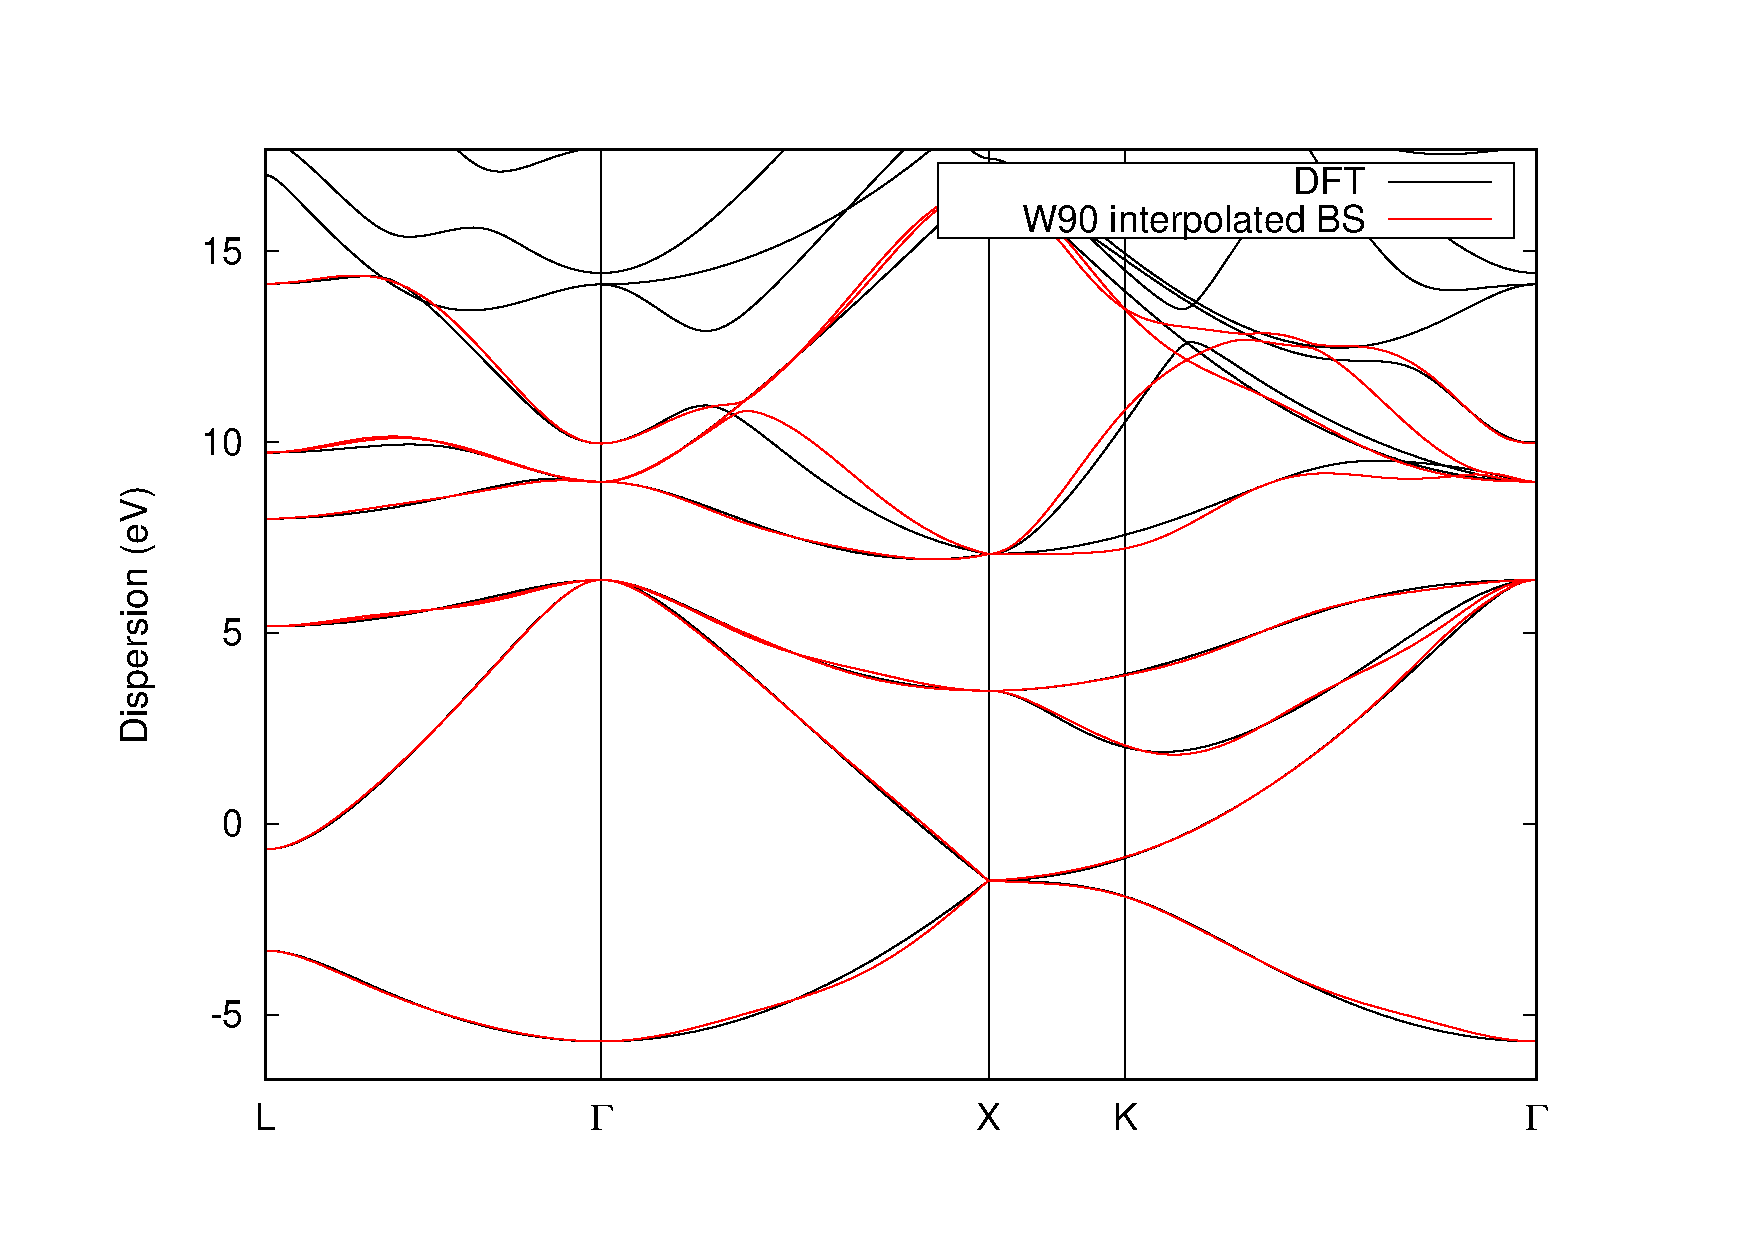
\includegraphics[width=0.7\columnwidth]{figure/example11/silicon_bandstructure.pdf}
\caption{Bandstructure of silicon from DFT calculation (solid black) and from Wannier interpolation (solid red).}\label{fig11.3}
\end{figure}
\end{itemize}

\subsection*{Further ideas}
\begin{itemize}
	\item {\it Compare the Wannier-interpolated bandstructure with the full pwscf bandstructure with a finer $k$-point grid.}

    Result for a $8\times8\times8$ mesh is shown in \Fig{fig11.4}.

	\begin{figure}[h!]
	\centering
	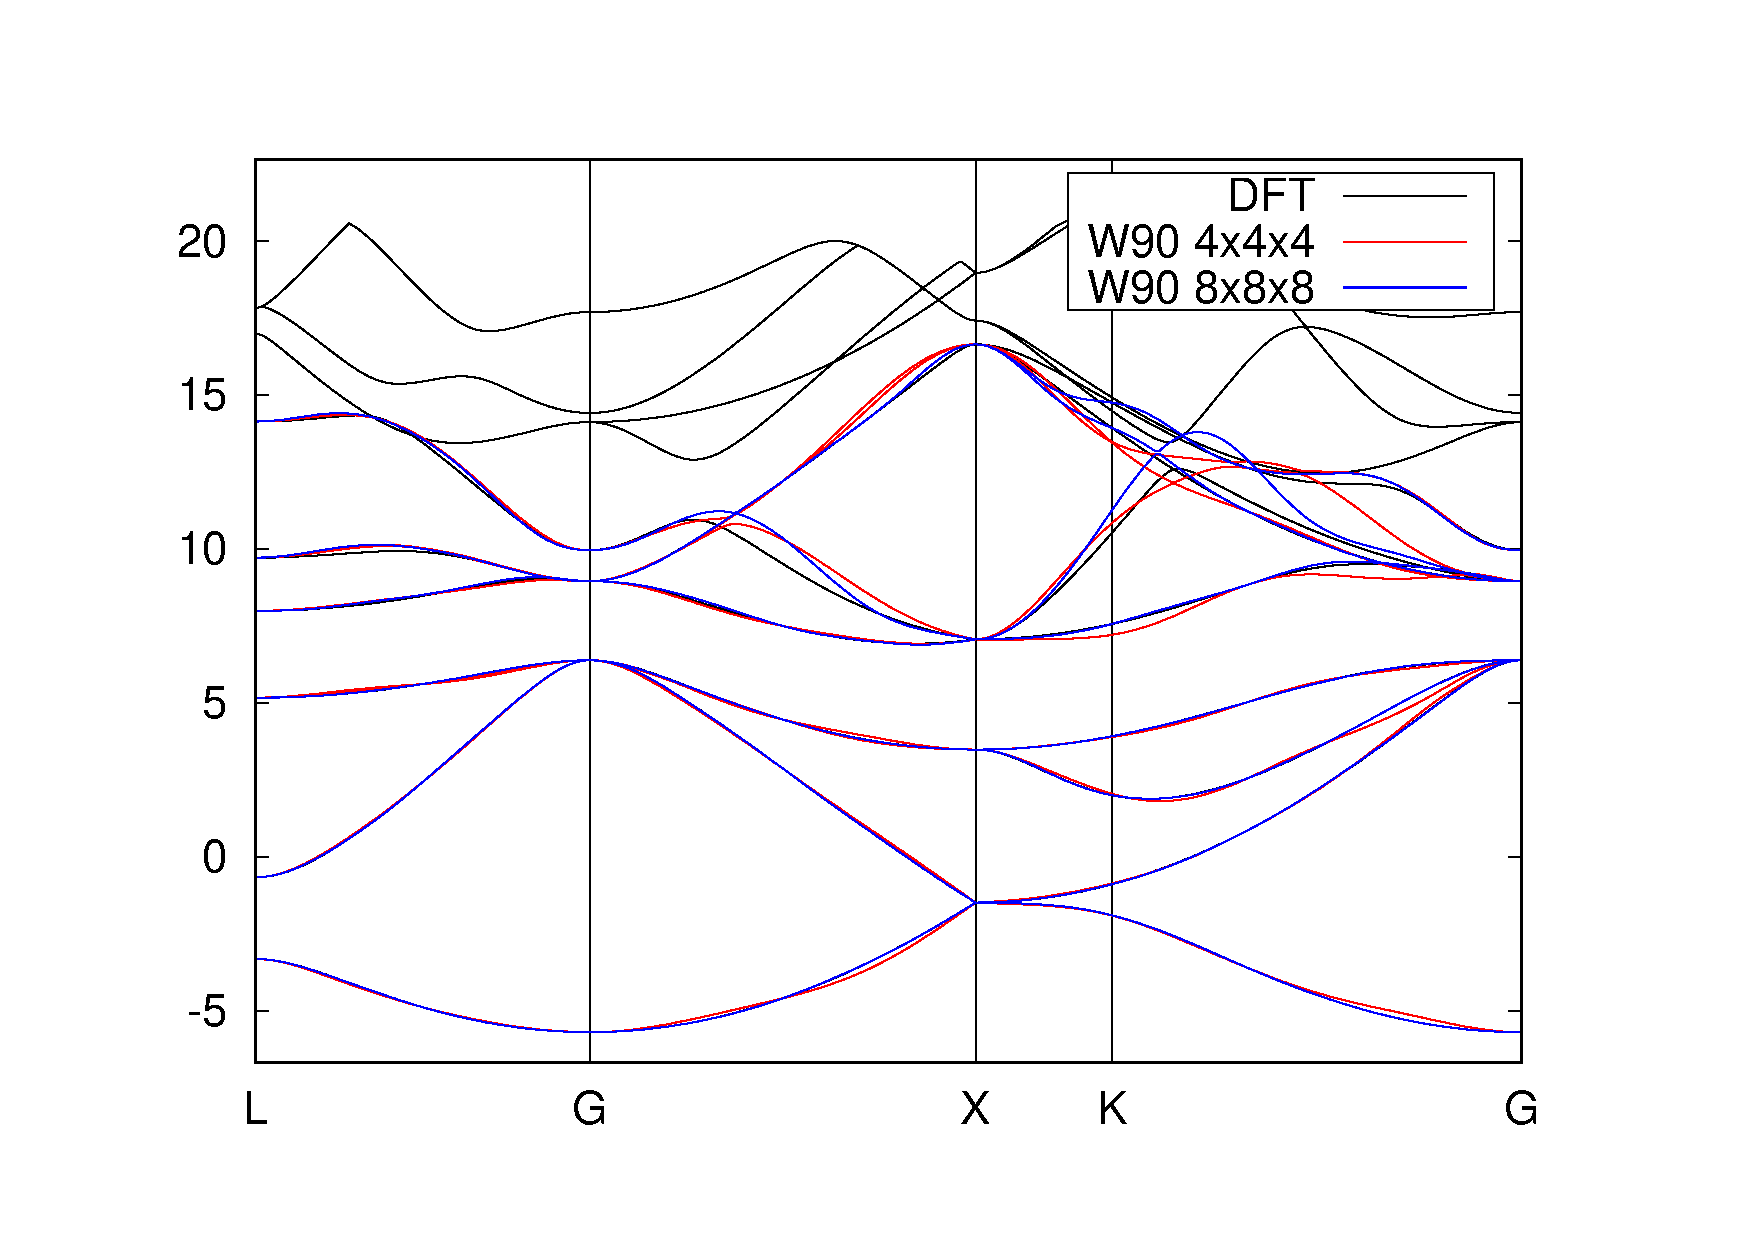
\includegraphics[width=0.7\columnwidth]{figure/example11/silicon_bs_DFT_vs_W90_finer_grid.pdf}
	\caption{Bandstructure of silicon from DFT calculation (solid black) and from Wannier interpolation with a $4\times4\times4$ mesh (solid red) and $8\times8\times8$ mesh (solid blue).}\label{fig11.4}
	\end{figure}

	\item {\it Compute four MLWFs spanning the low-lying conduction states.}

	The \MLWFs{} spanning the 4 low-lying conduction states are shown in \Fig{fig11.5}. The initial projections were 4 $sp3$ on the Si atom at (0,0,0).
	\begin{figure}[h!]
	\centering
	\subfloat[1]{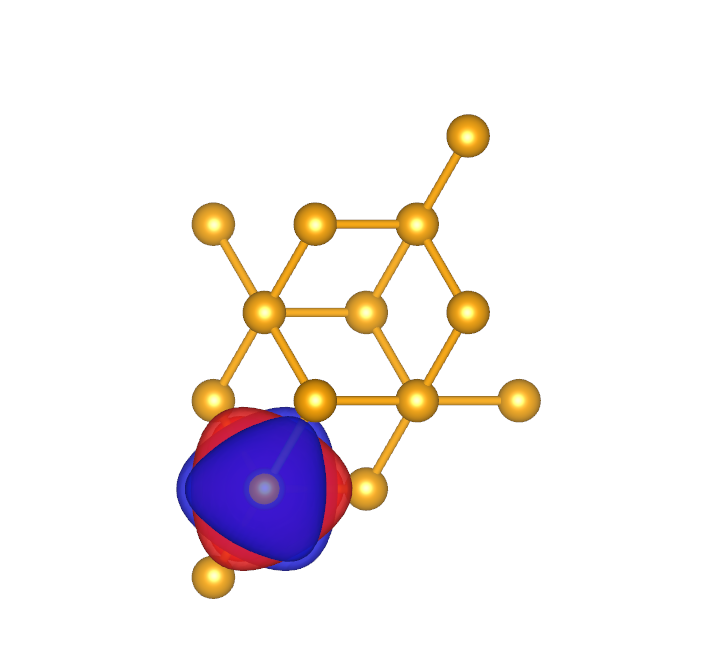
\includegraphics[width=0.25\columnwidth,trim={0pt 0pt 0pt 0pt},clip]{figure/example11/silicon_conduction_1.png}}
	\centering
	\subfloat[2]{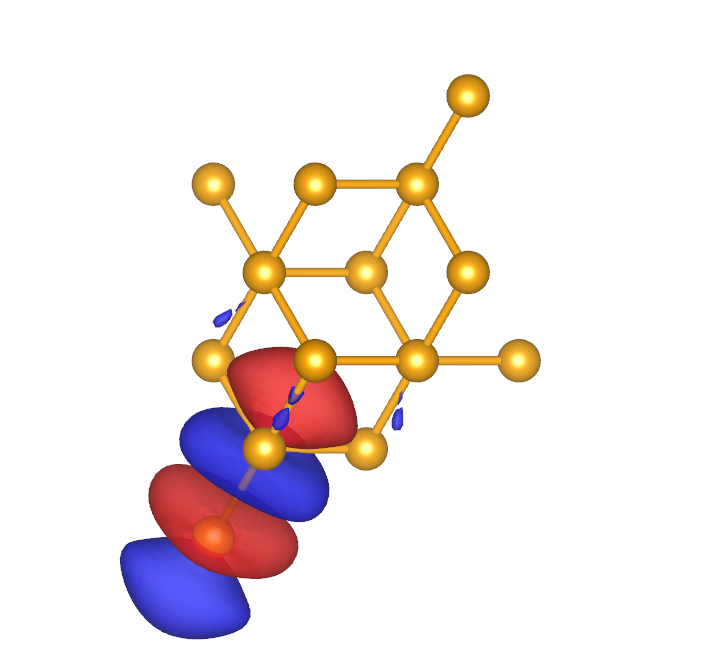
\includegraphics[width=0.25\columnwidth,trim={0pt 0pt 0pt 0pt},clip]{figure/example11/silicon_conduction_2.png}}
	\centering
	\subfloat[3]{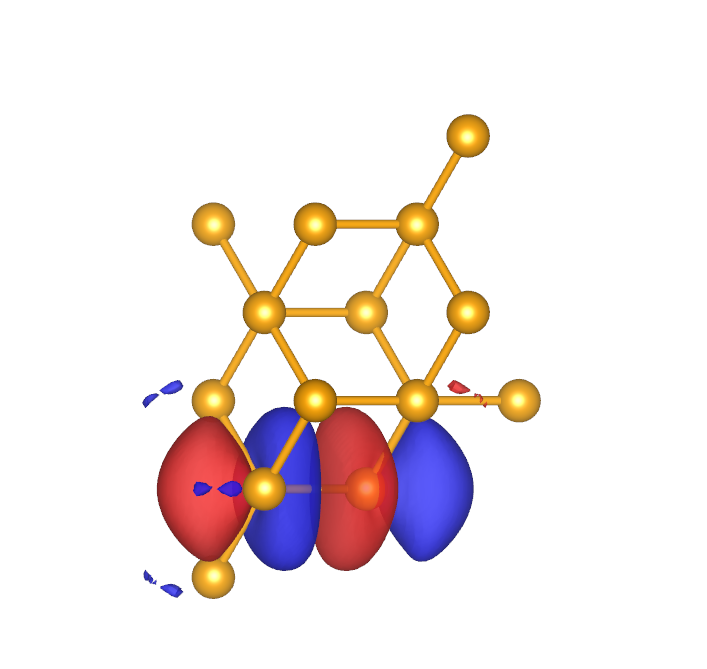
\includegraphics[width=0.25\columnwidth,trim={0pt 0pt 0pt 0pt},clip]{figure/example11/silicon_conduction_3.png}}
	\centering
	\subfloat[4]{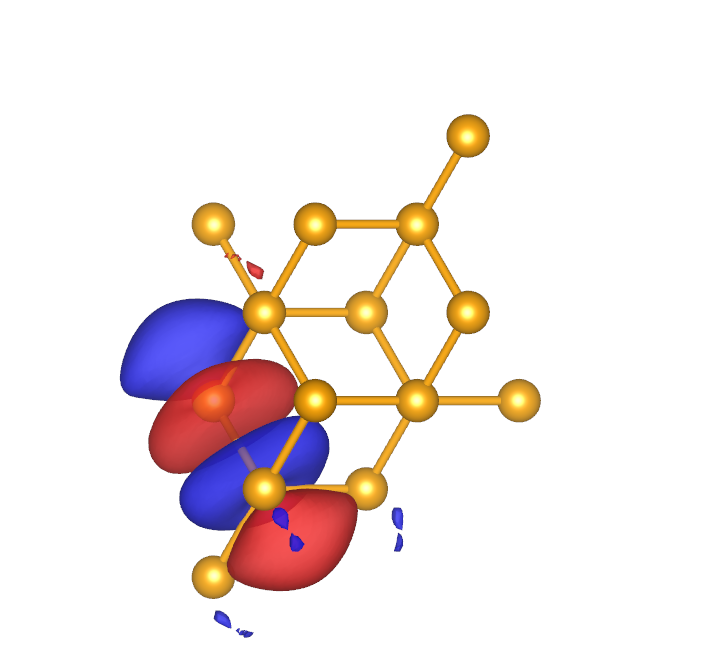
\includegraphics[width=0.25\columnwidth,trim={0pt 0pt 0pt 0pt},clip]{figure/example11/silicon_conduction_4.png}}
	\caption{}\label{fig11.5}
	\end{figure}
\end{itemize}
